\chapter{Interpretazione astratta}

L'interpretazione astratta è una tecnica di analisi statica che consiste nel definire un approssimazione \emph{corretta} e \emph{decidibile} della semantica del programma da analizzare. Compare per la prima volta nel paper \cite{cousot} di P.~Cousot e R.~Cousot del 1977. 

\section{Semantica}

\begin{definition}[Semantica]
La semantica di un programma $P$ è la descrizione formale di come il programma viene eseguito attraverso una macchina. Si denota con $\semantics{P}$. 
\end{definition}

I programmi scritti in linguaggi imperativi sono composti da istruzioni che vengono eseguite in sequenza. Ad ogni step di computazione, la macchina aggiorna una tabella detta \emph{memoria} di associazioni variabile\textrightarrow{}valore. 

La semantica che descrive i programmi dovrà formalizzare il concetto di \emph{esecuzione di una istruzione}. Una rappresentazione efficace è quella del \emph{control flow graph}.

\begin{definition}[Control flow graph]
Il control flow graph è un grafo $\struct{V, E \subseteq V \times V}$ tale che l'insieme $V = \set{Point}$ dei vertici sono i punti del programma e l'insieme $E$ degli archi è l'insieme delle istruzioni. 
\end{definition}

\begin{definition}[Sistema di transizioni]
Un \emph{sistema di transizioni} è una struttura $\struct{\mathbf{S}, \to}$ del programma $P$ dove $\mathbf{S}$ è un insieme di stati (``fotografie" della memoria in un certo istante) ed $\to$ è una relazione binaria tra stati tale che
\[ \sigma \to \sigma' \iff \sigma' \text{ è un possibile successore di } \sigma; \quad \sigma, \sigma' \in \mathbf{S} \]
\end{definition}
La relazione $\to$ formalizza il concetto di step di esecuzione. Una sequenza di stati $\sigma_0 \sigma_1 ... \sigma_n$ è detta \emph{trace}. Ogni trace rappresenta una esecuzione di un programma è può anche essere infinita. Da questa si può definire la \emph{trace semantics} (per approfondimenti vedi \cite{xavier}).

\subsection{Trace semantics}

\begin{definition}[Trace semantics]
Dato un sistema di transizioni $\struct{\mathbf{S}, \to}$ del programma $P$ è definita la trace semantics $\semantics{\mathbf{S}}$ come l'insieme delle possibili tracce di esecuzione di $P$:
\[ \semantics{\mathbf{S}} = \{ \sigma_0 \sigma_1 ... \sigma_n \mid \forall i \;\, \sigma_i \in \mathbf{S} \land (\sigma_i \to \sigma_{i+1}) \} \]
\end{definition}

Guardando la trace semantics possiamo vedere in ogni momento dell'esecuzione di un programma se una certa proprietà vale o no. Noi preferiremmo non essere legati alle informazioni temporali che porta con se la trace. Definiamo quindi una semantica che evidenzia le \emph{invarianti} presenti in ogni punto dell'esecuzione. 

\subsection{Collecting semantics}

\begin{definition}[Collecting semantics]
La collecting semantics di un programma $P$ rappresentato dal control flow graph $\struct{\set{Point}, E}$ è una funzione
\[ \mathcal{CS} : \set{Point} \to \wp(\set{State}) \]
che associa ad un punto del programma l'insieme dei possibili stati che può avere.
\end{definition}

Conoscendo la collecting semantics di $P$ possiamo facilmente verificare se la nostra proprietà vale o meno. $\mathcal{CS}$ può essere ricavata tramite un algoritmo di fixpoint iterativo (per approfondire vedi Sezione~\ref{sec:fixpoint}). 

\begin{example}\label{example:collecting}
Calcola la collecting semantics del seguente pezzo di codice.
\begin{javascriptcode}
x = 0;
y = 2;
while (x < 3) {
    y = y * y;
    x = x + 1;
}
\end{javascriptcode}
Lo stato che dobbiamo mantenere è una coppia $\struct{x,y}$ che all'inizio ha valore $\set{INIT} = \{ \struct{0, 2} \}$. La funzione di cui dobbiamo trovare il least fixed point è
\[ P(M) = \texttt{WHILE}_{x<3}(\texttt{INCX}(\texttt{SQUAREY}(M)), \set{INIT}) \]
con 
\begin{align*}
    \texttt{SQUAREY}(M) &= \{ \struct{x,y^2} \mid \struct{x,y} \in M \} \\
    \texttt{INCX}(M) &= \{ \struct{x+1,y} \mid \struct{x,y} \in M \} \\
    \texttt{WHILE}_{x<3}(M, I) &= (M \cup I) \cap \{ \struct{x,y} \mid x < 3 \} 
\end{align*}

Procediamo col metodo iterativo:
\begin{align*}
    P(\varnothing) 
        &= (\texttt{INCX}(\texttt{SQUAREY}(\varnothing)) 
        \cup \{ \struct{0, 2} \} ) 
        \cap \{ \struct{x,y} \mid x < 3 \} \\
        &= \{ \struct{0, 2} \} \\
    P(\{ \struct{0, 2} \}) 
        &= (\texttt{INCX}(\texttt{SQUAREY}(\{ \struct{0, 2} \})) 
        \cup \{ \struct{0, 2} \} ) 
        \cap \{ \struct{x,y} \mid x < 3 \} \\
        &= \{ \struct{0, 2},  \struct{1, 4} \} \\
    P(\{ \struct{0, 2},  \struct{1, 4} \}) 
        &= (\texttt{INCX}(\texttt{SQUAREY}(\{ \struct{0, 2},  \struct{1, 4} \})) 
        \cup \{ \struct{0, 2} \} ) 
        \cap \{ \struct{x,y} \mid x < 3 \} \\
        &= \{ \struct{0, 2},  \struct{1, 4}, \struct{2, 16} \} \\
    P(\{ \struct{0, 2},  \struct{1, 4}, \struct{2, 16} \} ) 
        &= (\texttt{INCX}(\texttt{SQUAREY}(\struct{0, 2},  \struct{1, 4}, \struct{2, 16})) 
        \cup \{ \struct{0, 2} \} ) 
        \cap \{ \struct{x,y} \mid x < 3 \} \\
        &= \{ \struct{0, 2},  \struct{1, 4}, \struct{2, 16}, \struct{3, 64} \}
        \cap \{ \struct{x,y} \mid x < 3 \} \\
        &= \{ \struct{0, 2},  \struct{1, 4}, \struct{2, 16} \}
\end{align*}

Il least fixed point è il valore di memoria $M = \{ \struct{0, 2},  \struct{1, 4}, \struct{2, 16} \}$.
\end{example}

La semantica collecting è però spesso indecidibile. Occorre trovare un modo per renderla decidibile. 

\section{Dominio astratto}

Nell'Esempio~\ref{example:collecting}, la computazione del least fiexed point può diventare molto costosa: gli elementi dell'insieme $M$ sono coppie di tipo $\Z \times \Z$ e il loro numero può velocemente esplodere. Cerchiamo un modo per approssimare $M$. 

\begin{definition}[Dominio]
Il \emph{dominio} è l'insieme dei valori che le variabili possono assumere all'interno dello store. 
\end{definition}

Al posto che mantenere di ogni valore il numero esatto $n \in \Z$, ne manteniamo solamente la parte di informazione che ci interessa.

\begin{example}\label{example:sign}
Il dominio dei segni è definito come segue:
\[ \set{Sign} = \{ \top, \oplus, \ominus, 0, \bot \} \]
dove $\top$ rappresenta un qualsiasi numero, $\oplus$ i numeri positivi o o nulli, $\ominus$ quelli negativi o nulli, $0$ il sono numero zero e $\bot$ nessun numero (usato come condizione d'errore, per esempio la divisione per zero). 
\end{example}

\begin{example}\label{example:interval}
Il dominio degli intervalli è definito come segue:
\[ \set{Interval} = \{ [l,h] \mid l,h \in \Z; \; l \le h \} \]
\end{example}

Entrambi i domini in Esempio~\ref{example:sign} e Esempio~\ref{example:interval} sono approssimazioni del dominio $\wp(\Z)$. I primi due prendono il nome di \emph{dominio astratto} mentre quest'ultimo è detto \emph{dominio concreto}. I domini devono formare una struttura di reticolo completo (per approfondire vedi Sezione~\ref{sec:reticoli}).

\subsection{Connessioni di Galois}\label{sec:galois-c}

Dobbiamo trovare un metodo per passare trasformare gli elementi del dominio concreto in elementi del dominio astratto e viceversa. 

\begin{definition}[Connessione di Galois]
Dati due poset $\struct{C, \le}$ e $\struct{A, \preceq}$, la coppia di funzioni $\struct{\alpha, \gamma}$ viene definita \emph{connessione di Galois} e si indica con 
\[ C \galois{\alpha}{\gamma} A \]
dove
\begin{itemize}
    \item[$C$:] insieme detto dominio concreto;
    \item[$\gamma$:] funzione monotona di concretizzazione $\gamma : A \to C$, $\forall c \in C : c \le \gamma(\alpha(c))$;
    \item[$A$:] insieme detto dominio astratto;
    \item[$\alpha$:] funzione monotona di astrazione $\alpha : C \to A$, $\forall a \in A : a \preceq \alpha(\gamma(a))$.
\end{itemize}
\end{definition}

\begin{example}
Per il dominio di Esempio~\ref{example:sign}, le funzioni $\alpha$ e $\gamma$ sono definite come segue:
\begin{align*}
    \alpha(\varnothing)                                   & = \bot                 &
    \gamma(\bot)                                          & = \varnothing          \\
    \alpha(\{0\})                                         & = 0                    &
    \gamma(0)                                             & = \{ 0 \}              \\
    \alpha(\{ x \mid \min x \ge 0 \}) & = \oplus          &
    \gamma(\oplus)                                        & = \{ x \mid x \ge 0 \} \\
    \alpha(\{ x \mid \max x \le 0 \}) & = \ominus         &
    \gamma(\ominus)                                       & = \{ x \mid x \le 0 \} \\
    \alpha(\{ x \mid \min x < 0 \land \max x > 0\})       & = \top                 &
    \gamma(\top)                                          & = \mathbb{Z}
\end{align*}
\end{example}

\begin{figure}[htbp]
    \centering
    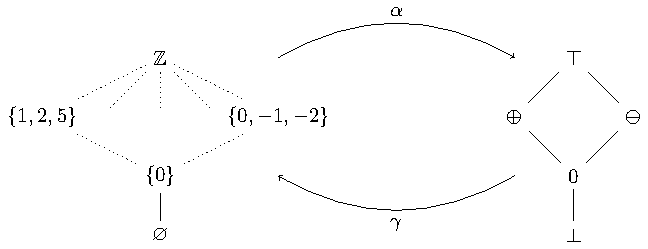
\includegraphics{capitoli/interpretazione-astratta/immagini/reticolo-segni.pdf}
    \caption{Connessione di Galois}
    \label{fig:galois-Z-sign}
\end{figure}

\subsection{Operazioni astratte}

Una volta definito il dominio astratto e la connessione di Galois, per ogni operazione $f : C \to C$ nel dominio concreto dobbiamo definire l'operazione $f^{\#} : A \to A$ nel dominio astratto. Il modo più immediato di definire $f^{\#}$ è tramite la \emph{best correct approximation}.

\begin{definition}[Best correct approximation]
Data una funzione $f : C \to C$ e una connessione di Galois $C \galois{\gamma}{\alpha} A$, si definisce $f^{\#} = \alpha \circ f \circ \gamma$ la \emph{best correct approximation} di $f$ in $A$.
\end{definition}

Tuttavia vorremmo poter avere il risultato di $f^{\#}$ senza dover eseguire $f$. Possiamo definire in un altro modo $f^{\#}$ e poi dimostrarne la correttezza.

\begin{definition}[Correttezza di una funzione astratta]
Data la connessione di Galois $C \galois{\gamma}{\alpha} A$ tra i due poset $\struct{C, \le}$ e $\struct{A, \preceq}$ ed una funzione concreta $f$, la funzione astratta $f^{\#}$ è un'approssimazione corretta di $f$ se vale
\[ \alpha \circ f = f^{\#} \circ \alpha \]
o equivalentemente
\[ f \circ \gamma = \gamma \circ f^{\#} \]
\end{definition}

\begin{example}
Consideriamo la funzione concreta $\fun{add} : \wp(\Z) \times \wp(\Z) \to \wp(Z)$:
\[ \fun{add}(X, Y) = \{ x + y \mid \forall x \in X, \, y \in Y \} \]
Per definire la sua funzione astratta nel dominio dei segni abbiamo più possibilità:
\[ \fun{add}^{\#}_1(s, t) = \alpha\big(\fun{add}(\gamma(s), \gamma(t)) \big) \]
oppure
\[ \fun{add}^{\#}_2(s,t) = \begin{array}{r|ccccc}
    s \downarrow; t \rightarrow & \top & \oplus & \ominus & 0       & \bot  \\\hline
    \top                      & \top   & \top   & \top    & \top    & \bot  \\
    \oplus                    & \top   & \oplus & \top    & \oplus  & \bot  \\
    \ominus                   & \top   & \top   & \ominus & \ominus & \bot  \\
    0                         & \top   & \oplus & \ominus & 0       & \bot  \\
    \bot                      & \bot   & \bot   & \bot    & \bot    & \bot  \\
\end{array} \]
oppure 
\[ \fun{add}^{\#}_3(s,t) = \top \]
Tutte e tre le varianti sono corrette. 
\end{example}









